\documentclass[10pt]{article}

% Margins and layout
\usepackage[left=0.75in,right=0.75in,top=0.8in,bottom=0.8in]{geometry}

% Encoding
\usepackage[T1]{fontenc}
\usepackage[utf8]{inputenc}

% Font package
\usepackage{times}

% No paragraph indent, less space between paragraphs
\setlength{\parindent}{0pt}
\setlength{\parskip}{0.7em}

% Page number in footer
\usepackage{fancyhdr}
\pagestyle{fancy}
\fancyhf{}
\cfoot{\thepage}
\renewcommand{\headrulewidth}{0pt}
\renewcommand{\footrulewidth}{0pt}

% Needed for [H] placement of figures
\usepackage{float}

% Graphics
\usepackage{graphicx}

% Optimize table layouts
\usepackage{booktabs}
\usepackage{array}
\usepackage{tabularx}

% Make links compact
\usepackage[colorlinks=true,linkcolor=blue,citecolor=blue]{hyperref}

% Math and bibliography
\usepackage[numbers]{natbib}
\usepackage{amsmath,amssymb}

% Make lists more compact
\usepackage{enumitem}
\setlist{noitemsep,topsep=2pt,parsep=0pt,partopsep=0pt}

% Column separation for two-column sections if needed
\usepackage{multicol}
\setlength{\columnsep}{0.5cm}

% More compact figure captions
\usepackage[font=small,labelfont=bf]{caption}

% More compact section titles
\usepackage{titlesec}
\titlespacing*{\section}{0pt}{1em}{0.5em}
\titlespacing*{\subsection}{0pt}{0.8em}{0.3em}
\titlespacing*{\subsubsection}{0pt}{0.6em}{0.2em}

\title{REPLACE WITH PAPER TITLE}
\author{Dian Gao, Anish Chandra, Linglong Meng}
\date{April 2025}

\begin{document}

\maketitle

\section{Introduction}

This study investigates how Large Language Model (LLM) agents can autonomously learn to use external memory systems when faced with sequential reasoning tasks. Prior research on memory-augmented agents has often relied on predefined memory architectures or hard-coded usage patterns, limiting the adaptability of such systems. Here, we explore a more flexible approach: equipping agents with multiple memory systems, minimal instructions, and allowing them to develop memory usage strategies that align with their objectives.

To create a controlled yet scalable environment for this exploration, we implement a self-play setup in TicTacToe. The environment ranges from the familiar $3 \times 3$ board to larger, more complex $6 \times 6$ and $9 \times 9$ boards. This scaling of the state space allows us to examine how memory usage strategies evolve with task complexity, and how different memory architectures support decision-making under varying conditions.

Our agents—built on the Cognitive Language Agent (CLA) framework—share the same underlying architecture, pairing OpenAI's GPT-4o-mini with external memory modules. However, they differ solely in their \textbf{prompt framing}: Agent A maximizes win rate without cost considerations, while Agent B balances win rate against token efficiency, explicitly guided by a win–token tradeoff formula and repeated reminders of memory costs. This setup isolates prompt-level guidance as the primary factor shaping agent behavior, holding architecture and task environment constant.

The agents interact with three complementary memory modalities: \textbf{GraphMemory} for structured, relational data; \textbf{VectorMemory} for similarity-based retrieval in embedding space; and \textbf{SemanticMemory} for conceptual storage (though SemanticMemory was only implemented for adaptive experiments and excluded from baseline and constrained settings due to time constraints). Through two experimental regimes—\textbf{constrained}, where agents are restricted to a single memory type, and \textbf{adaptive}, where agents can freely choose among available memory systems—we systematically evaluate how these architectures affect learning trajectories, scalability, and emergent strategies. Detailed logging of every memory call, token expenditure, and action rationale enables us to map memory usage patterns to agent performance.

Our results reveal significant differences in how agents deploy memory across architectures and objectives, offering new insights into designing adaptive, goal-driven memory systems for LLM agents operating in increasingly complex environments.

\section{Methods}

We evaluate our agents in a self-play TicTacToe environment, where two agents face off across varying board sizes ($3 \times 3$, $6 \times 6$, and $9 \times 9$). This setup offers a structured yet scalable domain for testing sequential reasoning, as the expansion of the board dramatically increases the state space and planning depth required for optimal play. The simplicity of TicTacToe facilitates clear interpretations of agent behavior, while the scaling provides a mechanism to probe memory demands under different levels of complexity.

Both agents in each game share a common architecture. Each is composed of a GPT-4o-mini core paired with external memory modules. The Cognitive Language Agent (CLA) framework guides this setup, combining a powerful language model with structured memory systems \cite{sumers2024cognitivearchitectureslanguageagents}. The key difference between the two agents lies in their objectives and prompt design. Agent A focuses on maximizing win rate without regard for efficiency, while Agent B balances winning with minimizing token use.

The agents interact with two primary types of external memory. \textbf{GraphMemory} organizes experiences as nodes and transitions, encoding structured relationships between game states. This architecture supports relational reasoning and enables the retrieval of paths through the game space. \textbf{VectorMemory}, by contrast, encodes states into fixed-dimensional embeddings via a simple autoencoder, facilitating similarity-based retrieval. This approach is better suited for pattern matching and generalization across loosely structured state spaces. While \textbf{SemanticMemory} was implemented only for adaptive experiments, providing conceptual storage capabilities and showing interesting usage patterns despite its limited implementation.

We conduct two main types of experiments. In the \textbf{constrained} setting, agents are restricted to a single memory type throughout a series of games. This isolates the effect of each architecture on performance, token usage, and memory behavior. In the \textbf{adaptive} setting, agents have access to all memory types and can choose which to use at each decision point. This allows us to probe whether agents can learn not only when to use memory, but which memory type to use depending on context.

For \textbf{baseline comparisons}, we evaluate memory-augmented agents against their no-memory counterparts. Each memory-enabled agent (Agent A or Agent B) is matched against an identical agent with memory modules disabled, isolating the effect of memory itself. Additionally, we compare Agent A without memory against Agent B without memory, providing a baseline for understanding the inherent effects of token efficiency tradeoffs without memory augmentation.

To ensure fair comparisons across agents, all experiments reset memory at the start of each experiment (spanning 15 or 30 games depending on the design). This design allows memory to persist across games within the same experiment, enabling us to examine whether LLM agents can leverage cross-game experiences to refine their strategies. By allowing memory carryover within experiments but not across them, we focus our analysis on within-experiment memory dynamics and learning behaviors. Throughout, we log token usage, memory calls, and agent rationales at each turn, enabling fine-grained insights into how memory strategies evolve under different conditions.

\subsection{The Agent: Agent A vs. Agent B}
Our agents are built on the Cognitive Language Agent (CLA) framework, combining a large language model (LLM) core with external memory systems to support long-term reasoning and strategy development \cite{sumers2024cognitivearchitectureslanguageagents}. The LLM used in this study is OpenAI's GPT-4o-mini, chosen for its balance between computational efficiency and expressive power. This architecture allows agents to integrate sequential experiences across games via external memory, while relying on the LLM for flexible reasoning.

\paragraph{Design Differences.}
Both agents share the same architecture and memory access mechanisms, but differ critically in their prompt framing and cost modeling, which jointly shape their memory usage strategies. While both agents are assigned the same explicit objective—maximize win rate while minimizing token usage—the underlying tradeoff parameter ($\lambda$) and prompt guidance diverge:

Agent A receives system prompts that focus purely on win rate maximization, with no mention of token costs or any tradeoff parameter. In effect, Agent A operates as if $\lambda = 0$.

Agent B, in contrast, is explicitly reminded of the token costs associated with memory operations. Its prompt specifies a concrete optimization formula:
$$
\text{maximize: win rate} - \lambda \times \text{token cost}
$$
where $\lambda$ governs the balance between winning and efficiency.

This design isolates the influence of implicit prompt guidance and cost sensitivity modeling. Although both agents nominally share the same objective in the system (maximize win rate while minimizing token use), Agent B receives additional framing and a defined $\lambda$, which lead it to adopt more conservative memory strategies. This subtle but crucial difference allows us to explore how LLM agents internalize tradeoffs between performance and resource efficiency.

\paragraph{Hypothesized Behavior.} This design allows us to investigate how \textbf{subtle variations in prompt framing}---rather than differing objective functions---shape emergent behaviors. We hypothesize that, even under a shared formal objective, agents will exhibit distinct memory usage patterns based on the implicit guidance embedded in their prompts:
\begin{itemize}[leftmargin=*,nosep]
    \item Agent A, unburdened by efficiency concerns, is expected to adopt a more \textbf{aggressive memory strategy}
    \item Agent B is encouraged toward \textbf{selective, resource-conscious behaviors}
\end{itemize}

\paragraph{Baseline Comparisons.}
To rigorously assess the influence of memory augmentation, we implement a structured set of baseline comparisons. For each agent type (Agent A and Agent B), we compare the performance of a memory-augmented agent against an identical agent with external memory modules fully disabled. These no-memory agents retain the same GPT-4o-mini core and system prompts as their memory-augmented counterparts, ensuring that any performance difference can be attributed solely to the presence or absence of external memory systems. This design isolates the marginal effect of memory under fixed agent configurations.

Beyond within-agent comparisons, we also conduct cross-agent baseline tests. Specifically, we compare \textbf{Agent A without memory} to \textbf{Agent B without memory}. This pairing enables us to evaluate whether the token-efficiency framing in Agent B's prompt affects decision quality even in the absence of memory. Since both agents share the same underlying model and are stripped of memory access, any performance divergence here reflects the impact of prompt-induced behavior under resource constraints.

In total, this baseline design enables three key contrasts:
\begin{enumerate}[leftmargin=*,nosep]
    \item \textbf{Memory-enabled vs. no-memory agents (within agent type)}: Isolating the performance lift due to memory architectures.
    \item \textbf{Agent A no-memory vs. Agent B no-memory}: Assessing token efficiency tradeoff effects in a memory-free setting.
\end{enumerate}

Experiments are conducted across two board sizes—$3 \times 3$ and $9 \times 9$—to capture the effects of task complexity on baseline dynamics. Each experimental condition runs for 15 games per pairing, balancing computational cost with statistical robustness. All baseline agents operate under the same memory-reset logic as their memory-augmented counterparts, ensuring comparability in experimental conditions.

\subsection{Memory Module Architecture}

To study the role of external memory in agent reasoning, we implement two complementary memory systems—\textbf{VectorMemory} and \textbf{GraphMemory}—each accessible via \verb|store| and \verb|retrieve| function bindings. These systems enable agents to record and recall experiences across game states, shaping their decision-making processes over time. A third system—\textbf{SemanticMemory}—was implemented only for adaptive experiments, providing conceptual storage capabilities and showing interesting usage patterns despite its limited implementation.

\paragraph{VectorMemory.} 
VectorMemory encodes each game state into a fixed-dimensional embedding, supporting similarity-based retrieval. Specifically, each $3 \times 3$ board is flattened into a 9-dimensional vector, which is passed through a simple autoencoder. The encoder compresses this input into a 6-dimensional latent space using a single linear layer with ReLU activation, while the decoder reconstructs the original input. Retrieval queries the memory with a current board state and returns the most similar stored vectors based on cosine similarity, facilitating pattern matching across structurally similar states. Metadata associated with each vectorized entry enables the agent to store strategic annotations alongside board configurations.

\paragraph{GraphMemory.}
GraphMemory organizes experiences as a directed graph, where each node represents a unique game state and edges encode transitions between states (moves). When an agent issues a retrieval query, it receives all immediate successor states and their metadata, providing a local relational context. This structure supports reasoning over sequential transitions and allows the agent to revisit past game paths.

\paragraph{Constrained vs. Adaptive Memory Use.}
We evaluate memory usage under two regimes. In \textbf{constrained} settings, agents are restricted to a single memory type (either GraphMemory or VectorMemory), enforced via system prompts and runtime checks that block disallowed memory operations. This isolates the impact of each memory architecture. In \textbf{adaptive} settings, agents have access to all available memory types and can choose which to use at each turn, enabling the exploration of emergent memory selection strategies.

\paragraph{Schema Updates.} 
In addition to \texttt{store} and \texttt{retrieve}, our memory systems expose a meta-memory operation, \texttt{updateSchema}, which allows agents to modify the structure or metadata schema of stored entries. While this functionality is implemented at the memory management layer, schema updates were \textbf{rarely invoked} in our experiments, as evidenced by empty schema update logs across all runs. This suggests that agents did not extensively engage in meta-memory reasoning under the current task setup, though the capability remains available for future studies exploring schema evolution.

\section{Results}

\subsection{Hypotheses}

Our hypotheses derive from two key design factors: the differing retrieval mechanisms of GraphMemory and VectorMemory, and the agents' contrasting objectives (win-maximizing vs. token-efficient). These considerations lead to the following hypotheses:

\begin{description}[itemsep=0.5em, parsep=0.5em]
\item[\textbf{H1.1}] \textit{VectorMemory supports better scalability than GraphMemory in large state spaces.} \\
Because VectorMemory retrieves based on similarity in embedding space, it can generalize across loosely structured states, whereas GraphMemory's reliance on relational transitions may struggle as the number of possible paths grows exponentially.

\item[\textbf{H1.2}] \textit{Memory usage frequency grows with task complexity, but the growth pattern differs across memory types.} \\
As the board size increases, agents are expected to rely more on memory to manage expanded state spaces. However, the degree of reliance should differ: GraphMemory's structural overhead may cap its usage, while VectorMemory's fuzzy retrieval allows more scalable engagement.

\item[\textbf{H2.1}] \textit{Win-maximizing agents (Agent A) will engage memory more aggressively than token-efficient agents (Agent B).} \\
Without cost constraints, Agent A should prioritize performance at any token cost, leading to more frequent memory calls. In contrast, Agent B's cost sensitivity should curb unnecessary memory usage.

\item[\textbf{H2.2}] \textit{Token-efficient agents (Agent B) will maintain higher win-rate-to-token ratios, reflecting more disciplined memory use.} \\
Even if raw win rates are lower, Agent B is expected to achieve better efficiency, optimizing for a balance between success and resource expenditure.

\item[\textbf{H3}] \textit{Adaptive agents will learn to prioritize VectorMemory over GraphMemory in complex environments.} \\
Given the scalability challenges of GraphMemory in large state spaces, we hypothesize that adaptive agents—when given a choice—will shift toward VectorMemory as task complexity grows.
\end{description}

In this section, we report findings from three experimental conditions---baseline (memory-free), constrained memory (fixed architecture), and adaptive memory selection---to investigate how memory architectures, agent objectives, and task complexity jointly shape agent behavior and performance. We evaluate agents across three board sizes ($3\times3$, $6\times6$, $9\times9$), examining win rate, token usage, and memory operation patterns.

\subsection{Baseline Performance: Memory-Free Agents}

The baseline condition evaluates agent performance in the absence of external memory, providing a reference point for understanding the intrinsic reasoning capabilities of the LLM across varying task complexities. Agent A and Agent B, with their differing prompt structures, face off across board sizes.

On the $3\times3$ board, Agent A achieves a win rate of \textbf{60.0\%}, while Agent B performs worse at \textbf{33.3\%}. This disparity suggests that the token-conscious framing of Agent B---which prompts the agent to consider token cost---negatively impacts its ability to compete, even in simple environments.

However, as board size increases, the performance gap flips. On the $9\times9$ board, Agent B dominates with a win rate of \textbf{80.0\%}, while Agent A drops to \textbf{20.0\%}. This inversion suggests that Agent A's lack of cost-awareness may lead to inefficient reasoning under high complexity, whereas Agent B's token-efficient strategy enables more scalable performance.

Notably, the overall \textbf{completion rate} on the $9\times9$ board drops to \textbf{66.7\%}, with \textbf{33.3\%} of games timing out due to LLM struggles in larger state spaces. This reinforces the need for external memory to support reasoning at scale.

\begin{figure}[H]
\centering
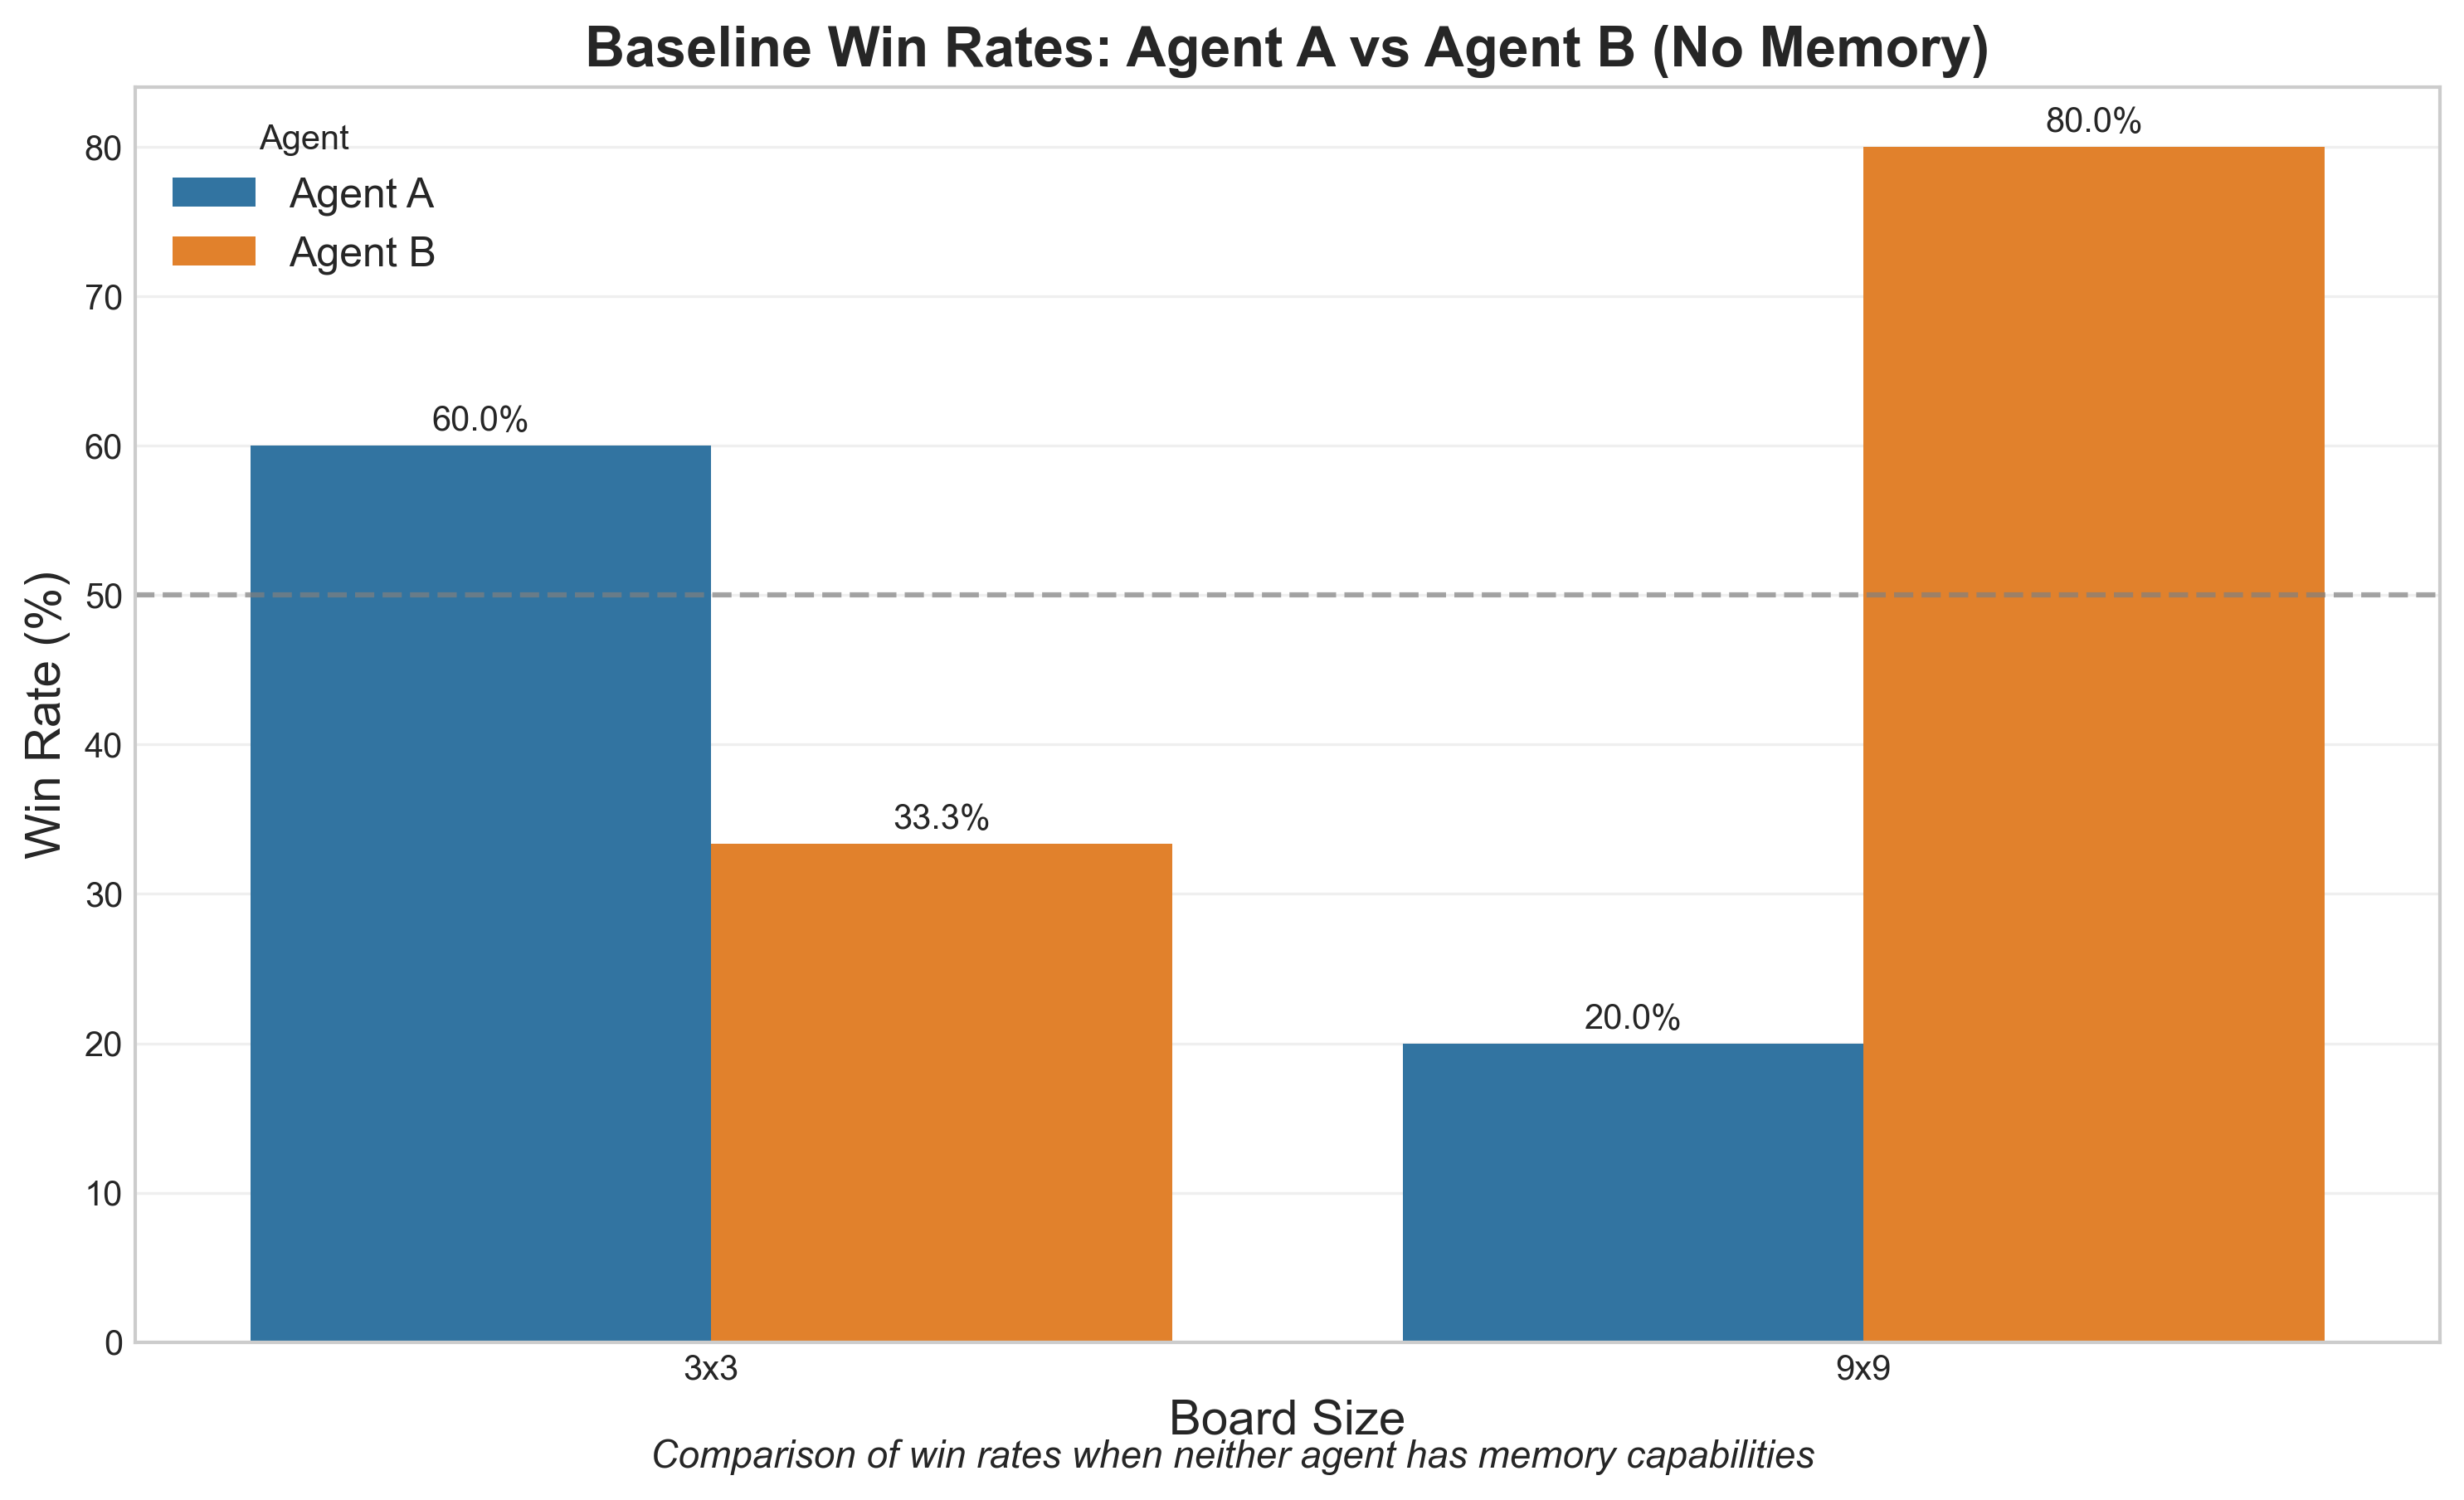
\includegraphics[width=0.6\textwidth]{figures/memory_baseline/baseline_win_rates.png}
\caption{Baseline win rates for Agent A and Agent B across board sizes (no memory).}
\label{fig:baseline_win_rates}
\end{figure}

To further illustrate the importance of memory augmentation, we compare each agent's performance with and without memory. As shown in Figure~\ref{fig:memory_baseline_comparison}, memory-augmented agents generally outperform their no-memory counterparts across both GraphMemory and VectorMemory settings, particularly in smaller board environments ($3\times3$) where memory retrieval remains lightweight. This performance lift confirms that external memory helps stabilize reasoning and mitigate LLM struggles in complex decision-making.

To further examine the impact of memory architectures, Figure~\ref{fig:baseline_complete_results} reports the complete win/draw/loss breakdowns for each agent across GraphMemory and VectorMemory conditions. These results reveal that while VectorMemory consistently boosts win rates and reduces losses for both agents, GraphMemory's effects are more variable—improving outcomes for Agent A but showing limited gains for Agent B.

\begin{figure}[H]
\centering
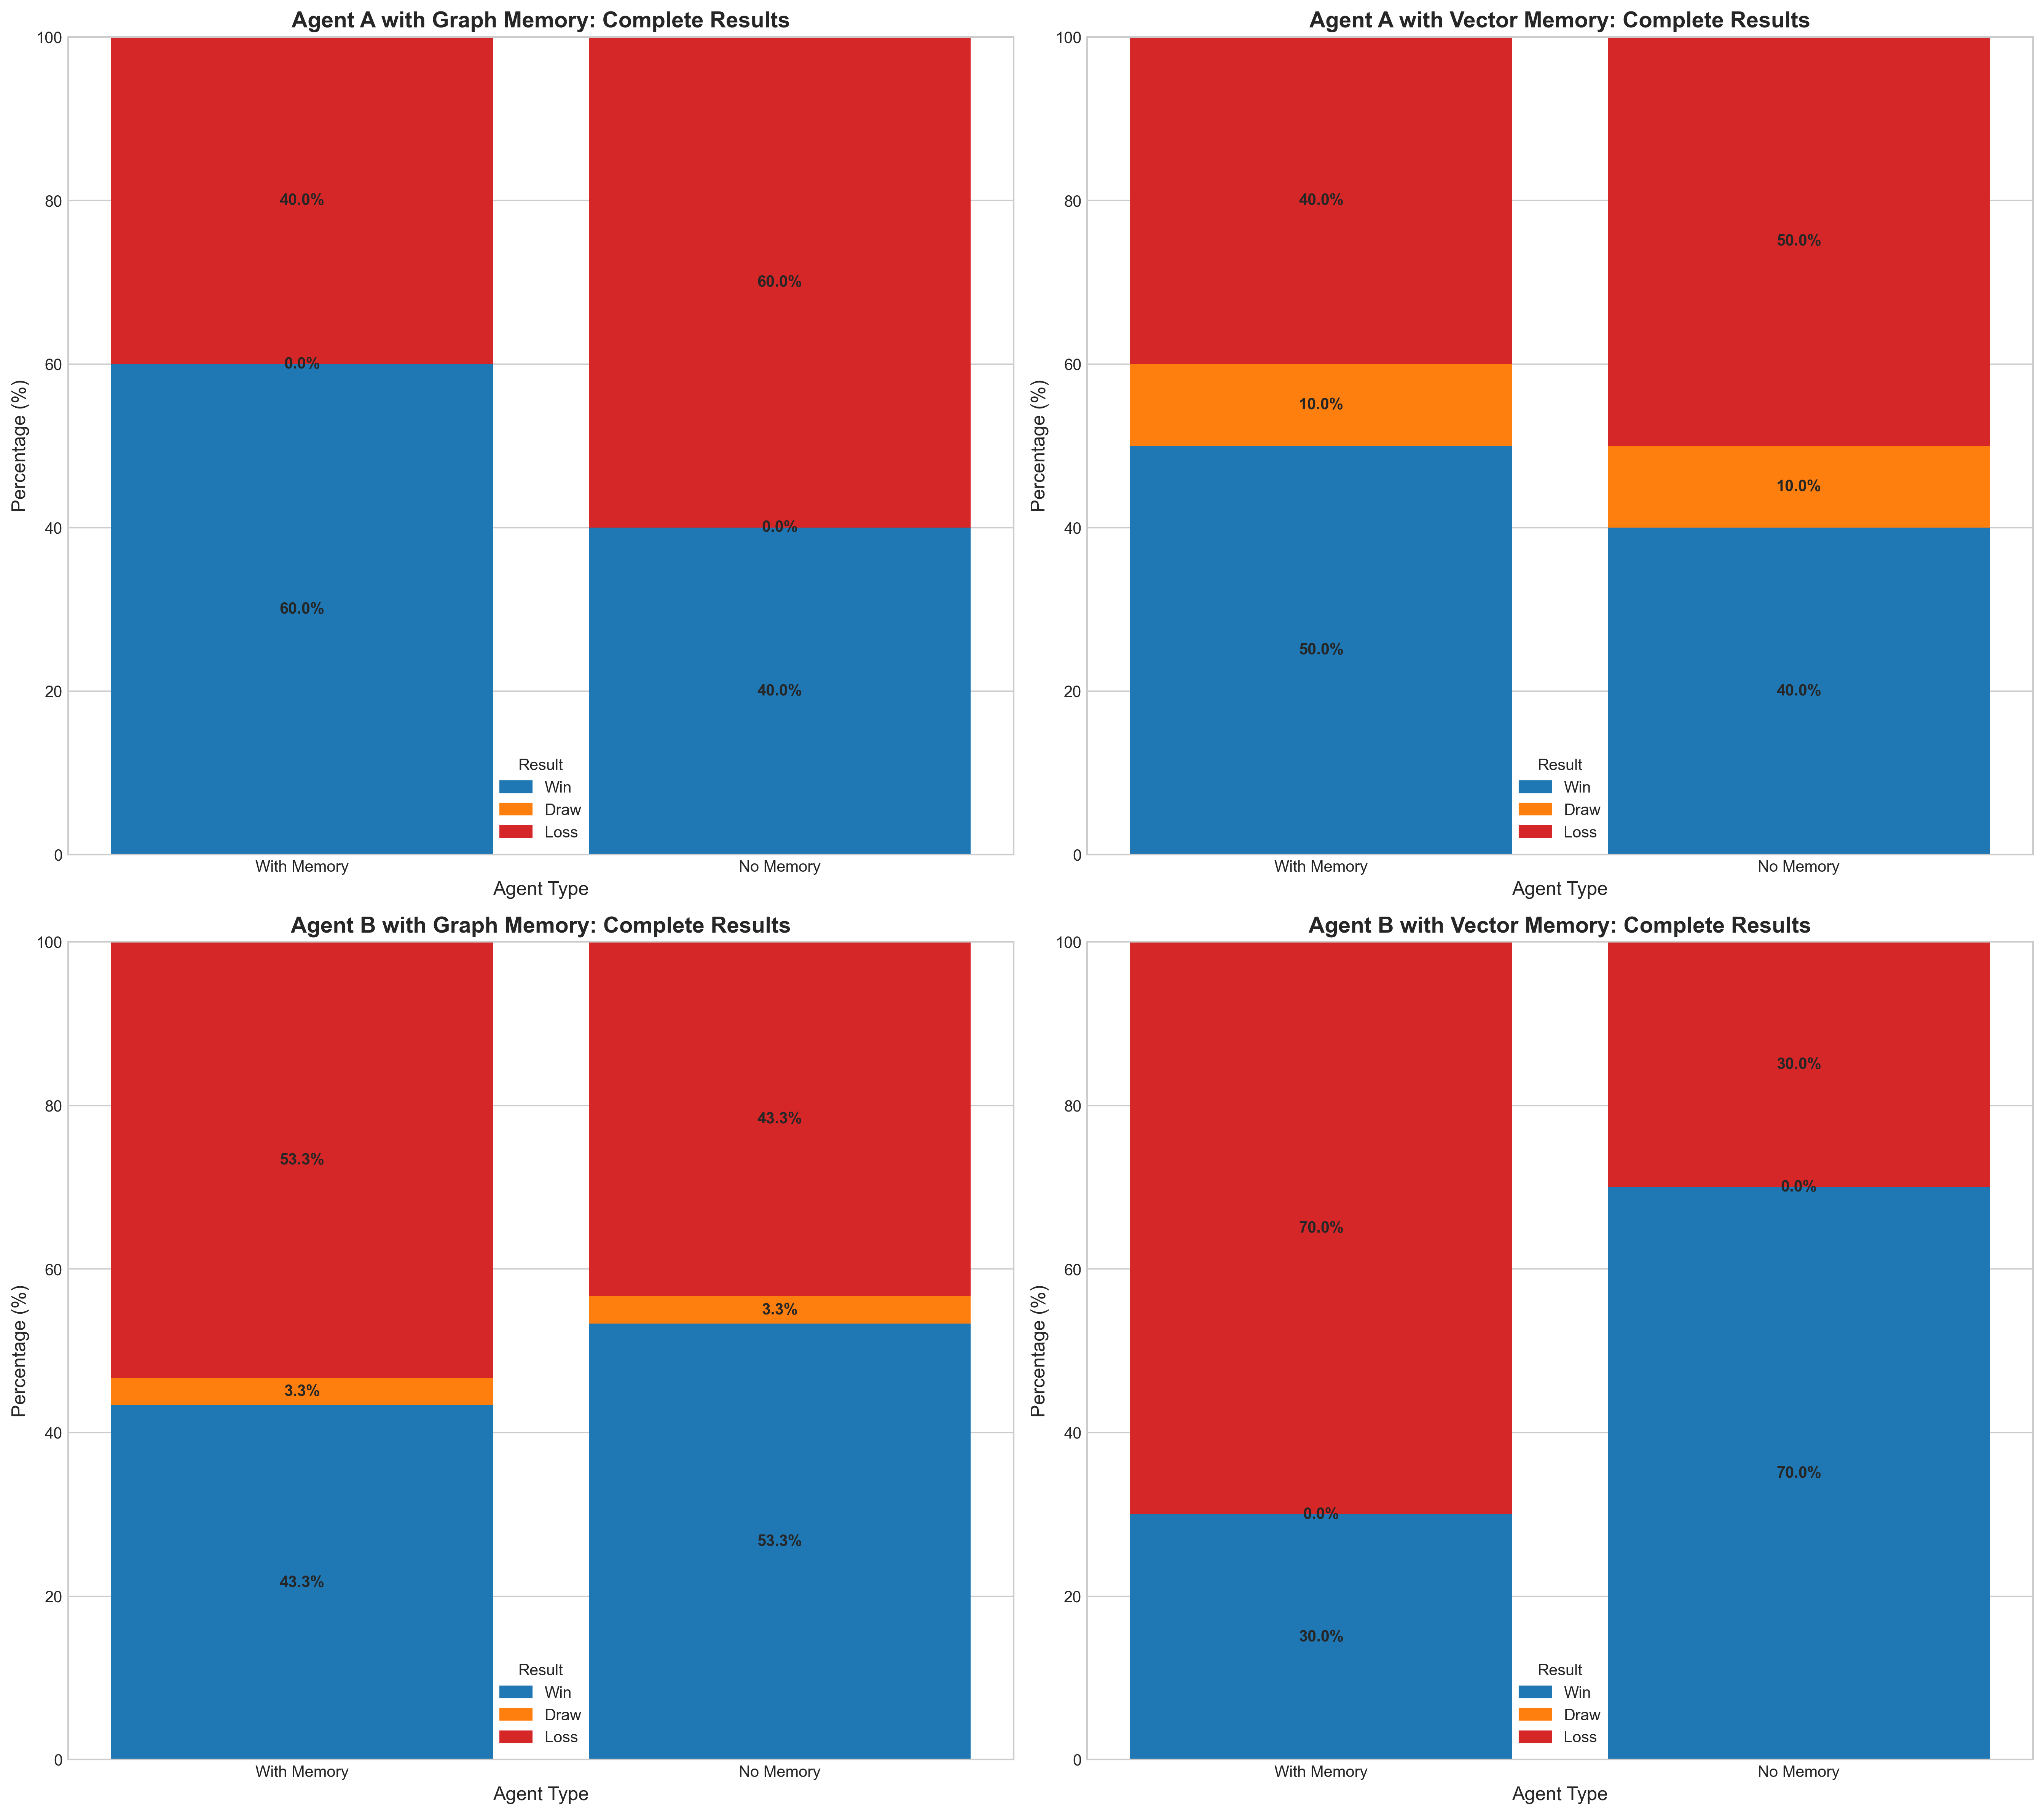
\includegraphics[width=0.6\textwidth]{figures/memory_baseline/memory_complete_results.png}
\caption{Complete game results (win/draw/loss breakdown) for Agent A and Agent B across memory types (GraphMemory vs. VectorMemory) in baseline comparisons. Memory-augmented agents (left bars) show improved win rates, especially with VectorMemory.}
\label{fig:baseline_complete_results}
\end{figure}

However, for both agents on $9\times9$ boards, this trend does not consistently hold. For \textbf{Agent A}, with-memory performance actually lags behind no-memory baselines, while \textbf{Agent B} shows only marginal gains. This counterintuitive result reflects both \textbf{design logic} and \textbf{data-level factors}. Agent A, driven solely by win maximization, adopts aggressive memory usage patterns. While this strategy leverages fast, similarity-based retrieval in VectorMemory, it suffers under GraphMemory's relational overhead in large state spaces, where token costs and retrieval complexity increase. Since the aggregated results in Figure~\ref{fig:memory_baseline_comparison} combine both memory architectures, GraphMemory's performance bottleneck drags down overall with-memory outcomes for Agent A at scale.

For Agent B, despite token-efficient prompting leading to more selective memory engagement, the conservative strategy may under-utilize retrieval opportunities in complex environments like $9\times9$, limiting performance benefits from memory.

These findings underscore a critical insight: \textbf{memory augmentation alone is insufficient without appropriate architectural choices and alignment with agent objectives}. Effective memory strategies must balance retrieval efficiency, task complexity, and the agent's optimization framing. Without this alignment, even well-designed memory systems can become performance bottlenecks in large decision spaces.

\begin{figure}[H]
\centering
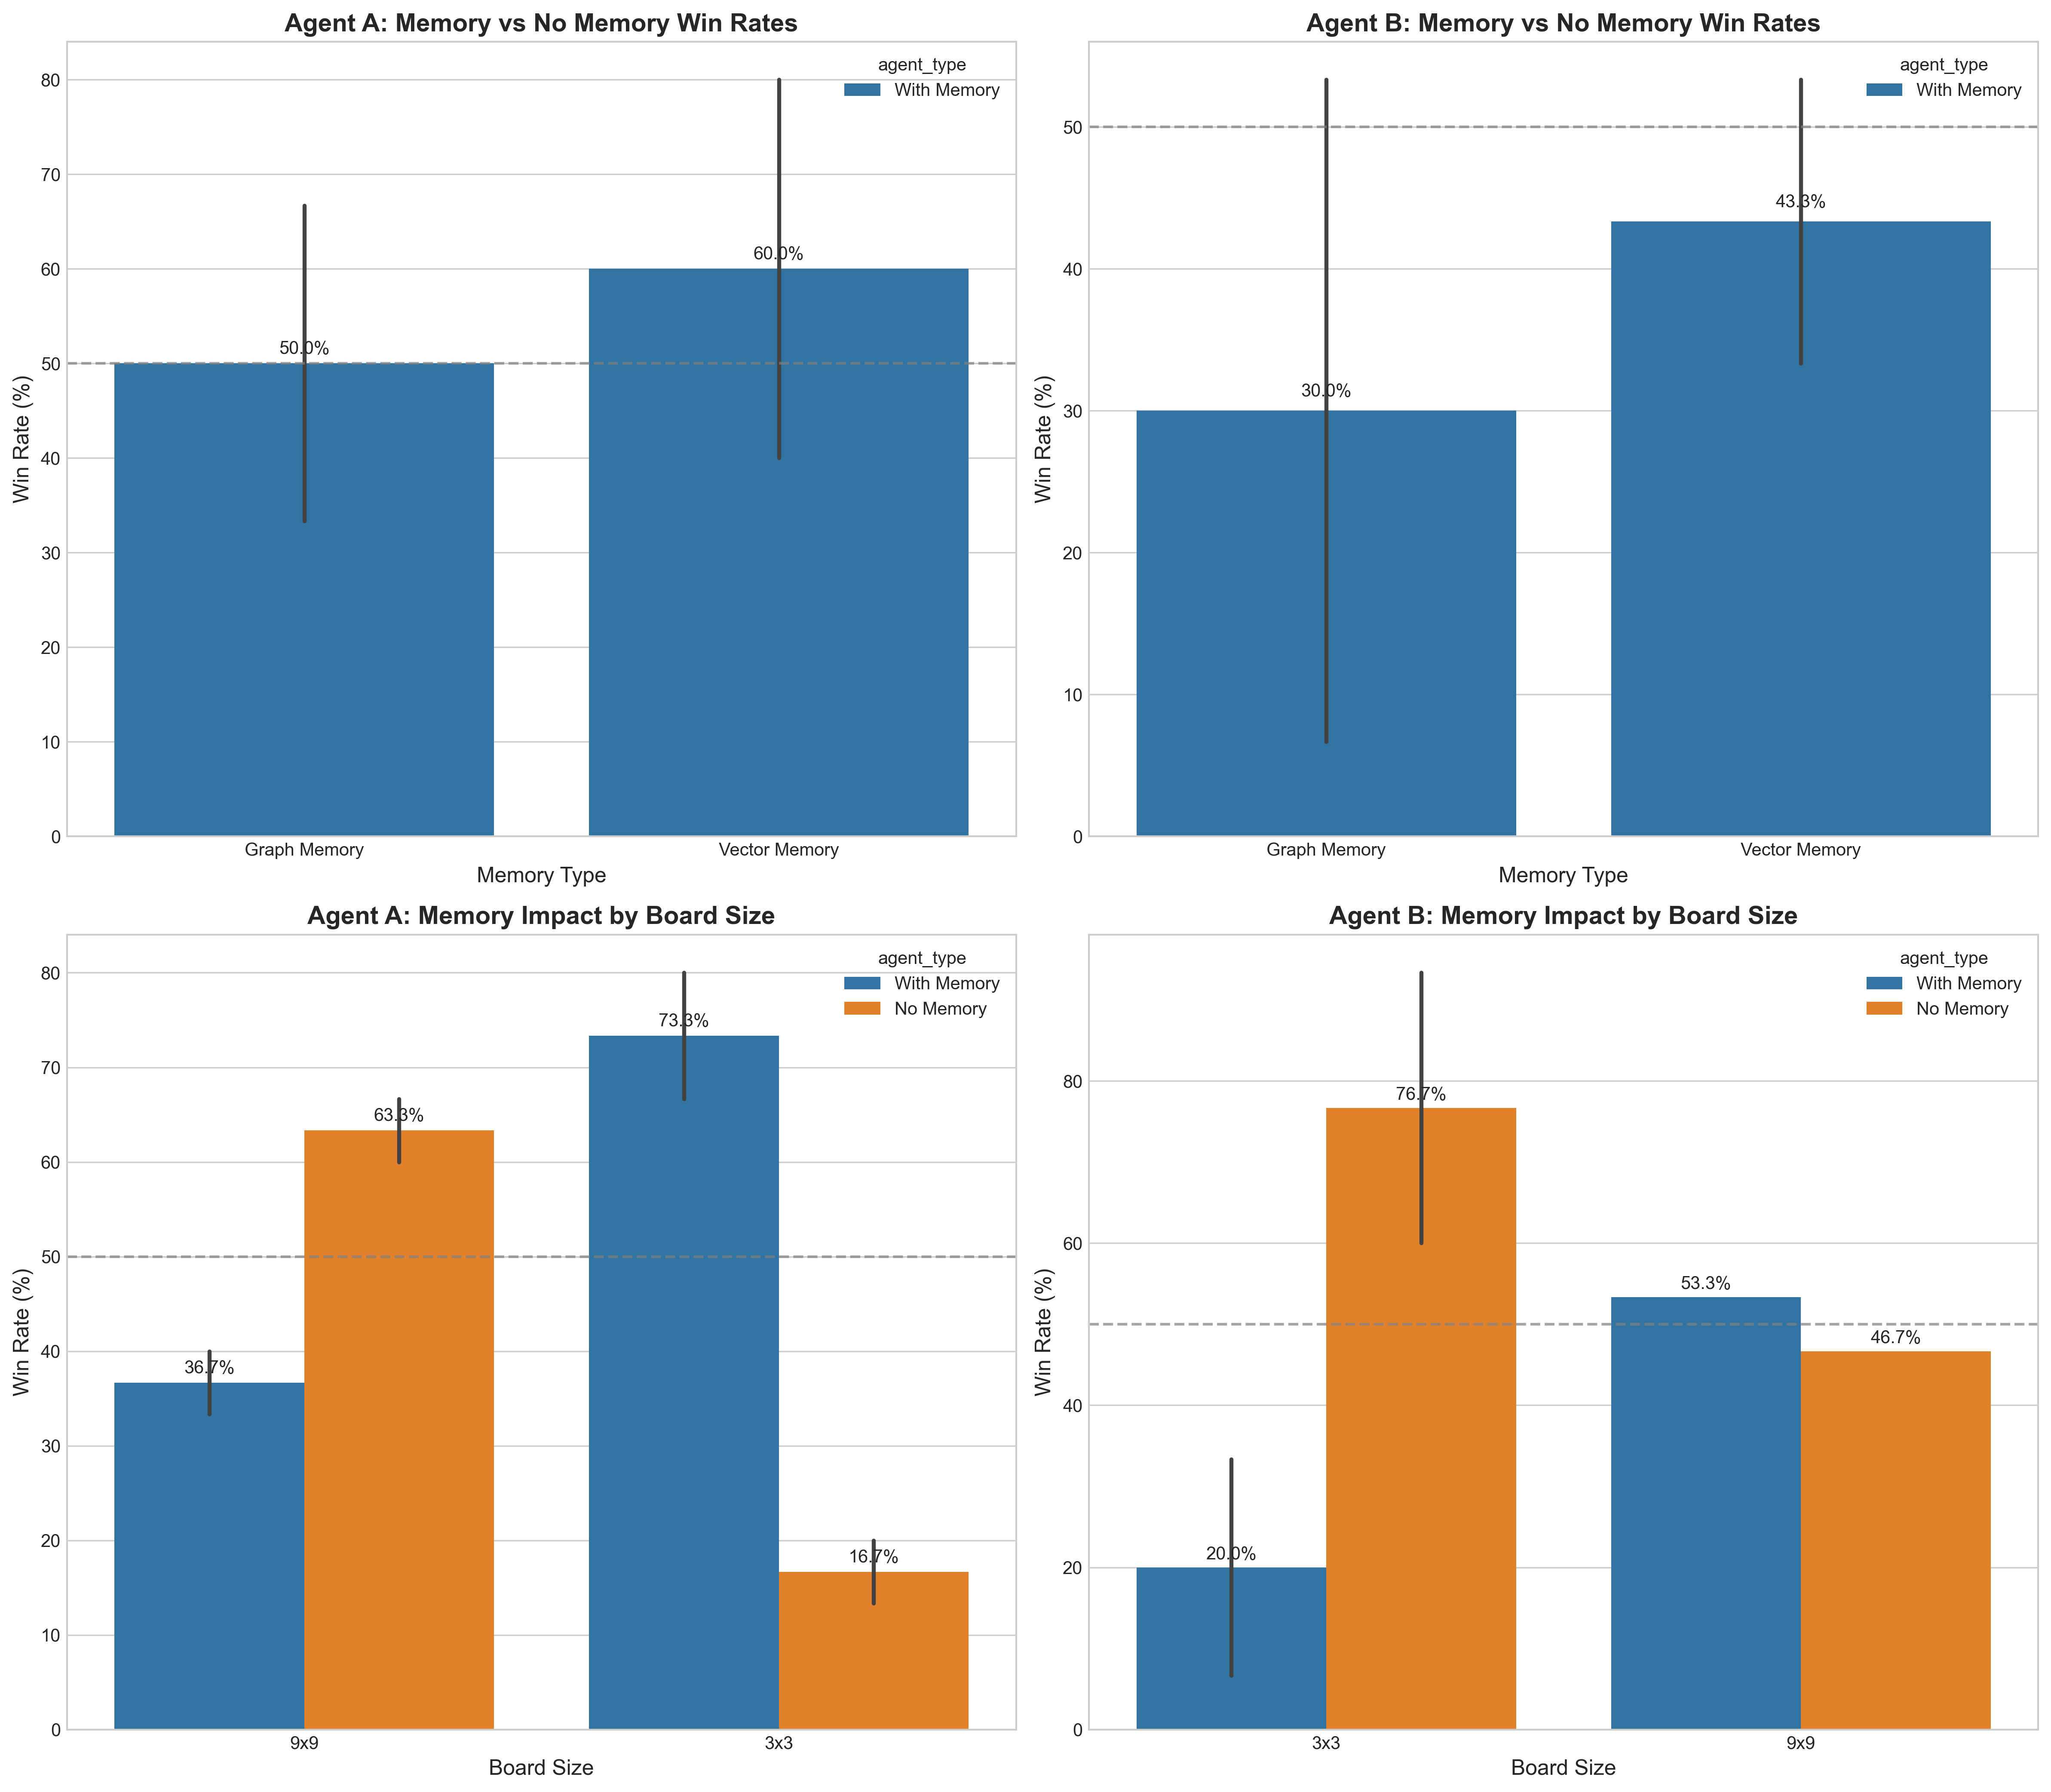
\includegraphics[width=0.7\textwidth]{figures/memory_baseline/memory_baseline_comparison.png}
\caption{Performance comparison within each agent: win rates with and without memory. Memory augmentation provides clear benefits across memory types and board sizes.}
\label{fig:memory_baseline_comparison}
\end{figure}

These findings establish two key points: 
\begin{enumerate}[leftmargin=*,nosep]
    \item Token-conscious prompting (Agent B) incurs a performance penalty in simple settings but demonstrates more scalable reasoning patterns in complex environments, though not always outperforming baseline agents without memory.
    \item External memory is critical for supporting reasoning at scale, but its effectiveness depends on architecture selection and alignment with agent strategies.
\end{enumerate}

\subsection{Constrained Memory Experiments}

\subsubsection{RQ1: Memory Architecture Effectiveness}

To assess how different memory architectures influence performance, we compare GraphMemory and VectorMemory under constrained conditions, where agents are restricted to a single memory type. Table~\ref{tab:winrates} reports win rates for both agents across board sizes and memory types.

\begin{table}[h]
\centering
\small
\caption{Win and draw rates across constrained memory types and board sizes.}
\begin{tabular}{@{}llccc@{}}
\toprule
Board Size & Memory Type & Agent A Win Rate & Agent B Win Rate & Draw Rate \\
\midrule
$3 \times 3$ & Graph  & 60.0\% & 20.0\% & 20.0\% \\
$6 \times 6$ & Graph  & 46.7\% & 53.3\% & 0.0\% \\
$9 \times 9$ & Graph  & 26.7\% & 73.3\% & 0.0\% \\
$3 \times 3$ & Vector & 66.7\% & 6.7\%  & 26.7\% \\
$6 \times 6$ & Vector & 60.0\% & 40.0\% & 0.0\% \\
$9 \times 9$ & Vector & 53.3\% & 46.7\% & 0.0\% \\
\bottomrule
\end{tabular}
\label{tab:winrates}
\end{table}

GraphMemory supports competitive performance on small boards, with Agent A achieving a \textbf{60.0\%} win rate on $3\times3$. However, as board size increases, GraphMemory's performance degrades significantly, with Agent A's win rate dropping to \textbf{26.7\%} on $9\times9$. Conversely, VectorMemory maintains more stable performance, with Agent A achieving \textbf{53.3\%} win rate on $9\times9$. This pattern supports \textbf{H1.2}, suggesting that VectorMemory's similarity-based retrieval scales more effectively as the state space expands.

\begin{figure}[ht]
\centering
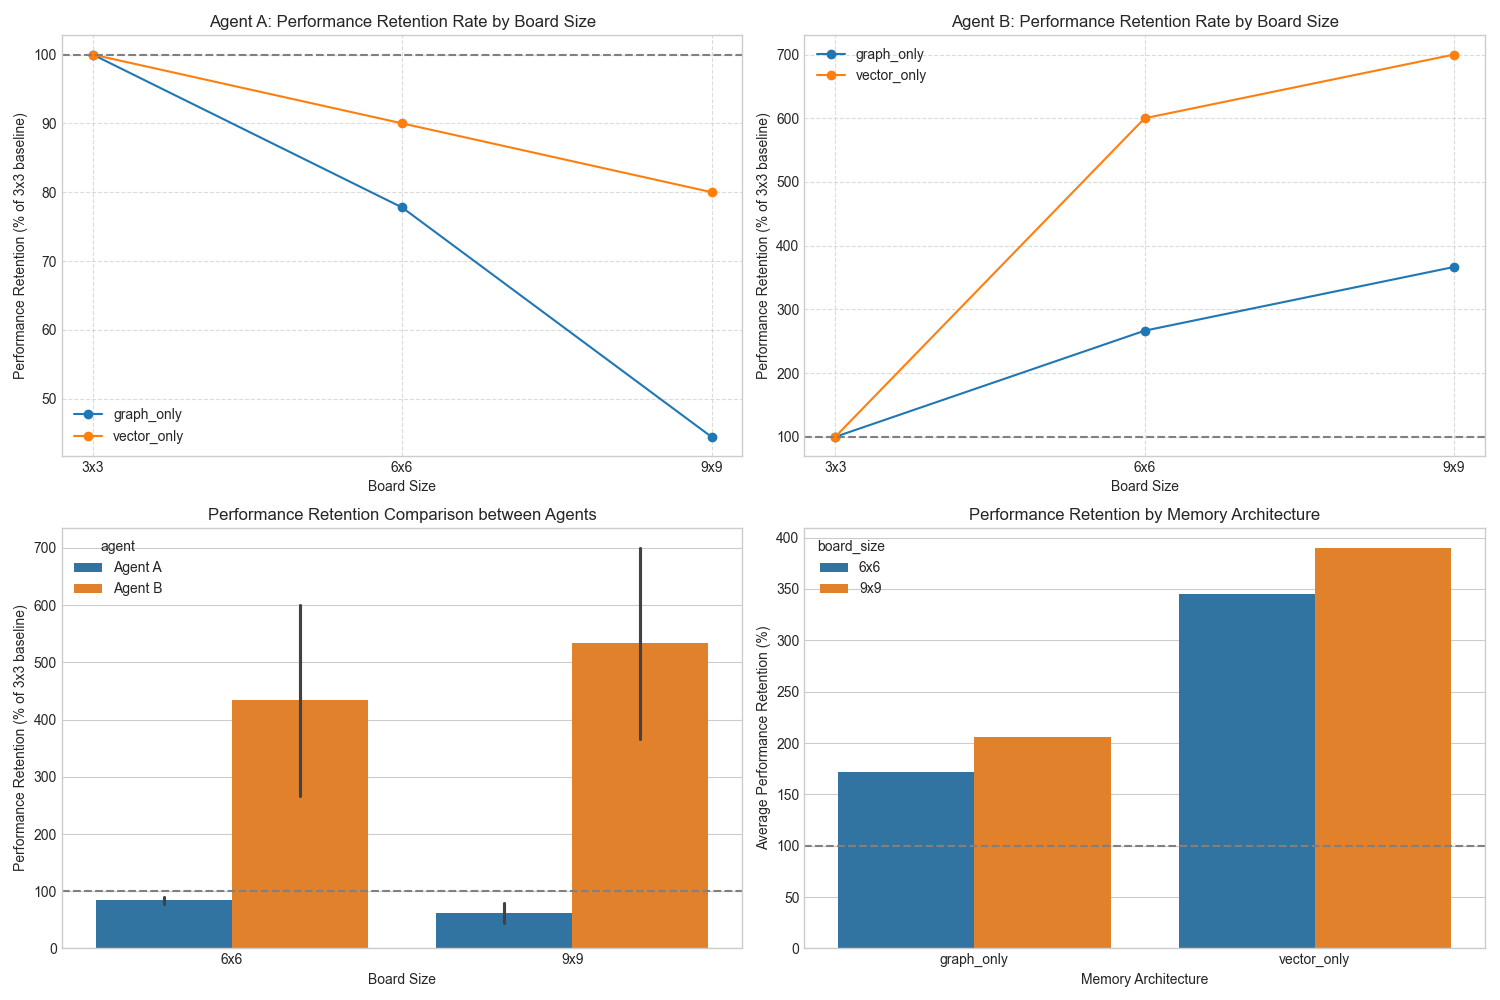
\includegraphics[width=0.7\textwidth]{figures/performance_retention_analysis.png}
\caption{Performance retention analysis (normalized win rates relative to $3\times3$).}
\label{fig:performance_retention}
\end{figure}

As shown in Figure~\ref{fig:performance_retention}, retention plots reveal that for Agent A, VectorMemory preserves approximately \textbf{80\%} of its baseline win rate on $9 \times 9$, while GraphMemory retention drops below \textbf{50\%}. For Agent B, although absolute win rates are higher, VectorMemory similarly maintains superior retention compared to GraphMemory. This supports \textbf{H1.2}, confirming that VectorMemory's similarity-based retrieval generalizes better in larger state spaces.

\subsubsection{RQ2: Memory Usage Growth with Complexity}

To investigate how memory usage scales with task complexity, we track the number of memory function calls per game across agents, memory types, and board sizes.

VectorMemory usage exhibits a \textbf{monotonic increase} in memory calls as board size grows, with Agent A's calls rising from \textbf{4} on $3\times3$ to \textbf{20} on $9\times9$. GraphMemory, in contrast, shows \textbf{non-linear growth}: memory calls peak at $6\times6$ (\textbf{21} calls for Agent A) but drop on $9\times9$ (\textbf{12} calls). This irregular pattern suggests diminishing returns from GraphMemory in larger, less structured state spaces. Agent A consistently makes \textbf{2--4 times more memory calls} than Agent B, reinforcing \textbf{H2.1} that win-maximizing agents are more liberal in memory usage. Agent B, constrained by token efficiency, remains more conservative. Figure~\ref{fig:memory_calls} illustrates these patterns, highlighting the distinct scaling behaviors of GraphMemory and VectorMemory across agents and board sizes.

\begin{figure}[ht]
\centering
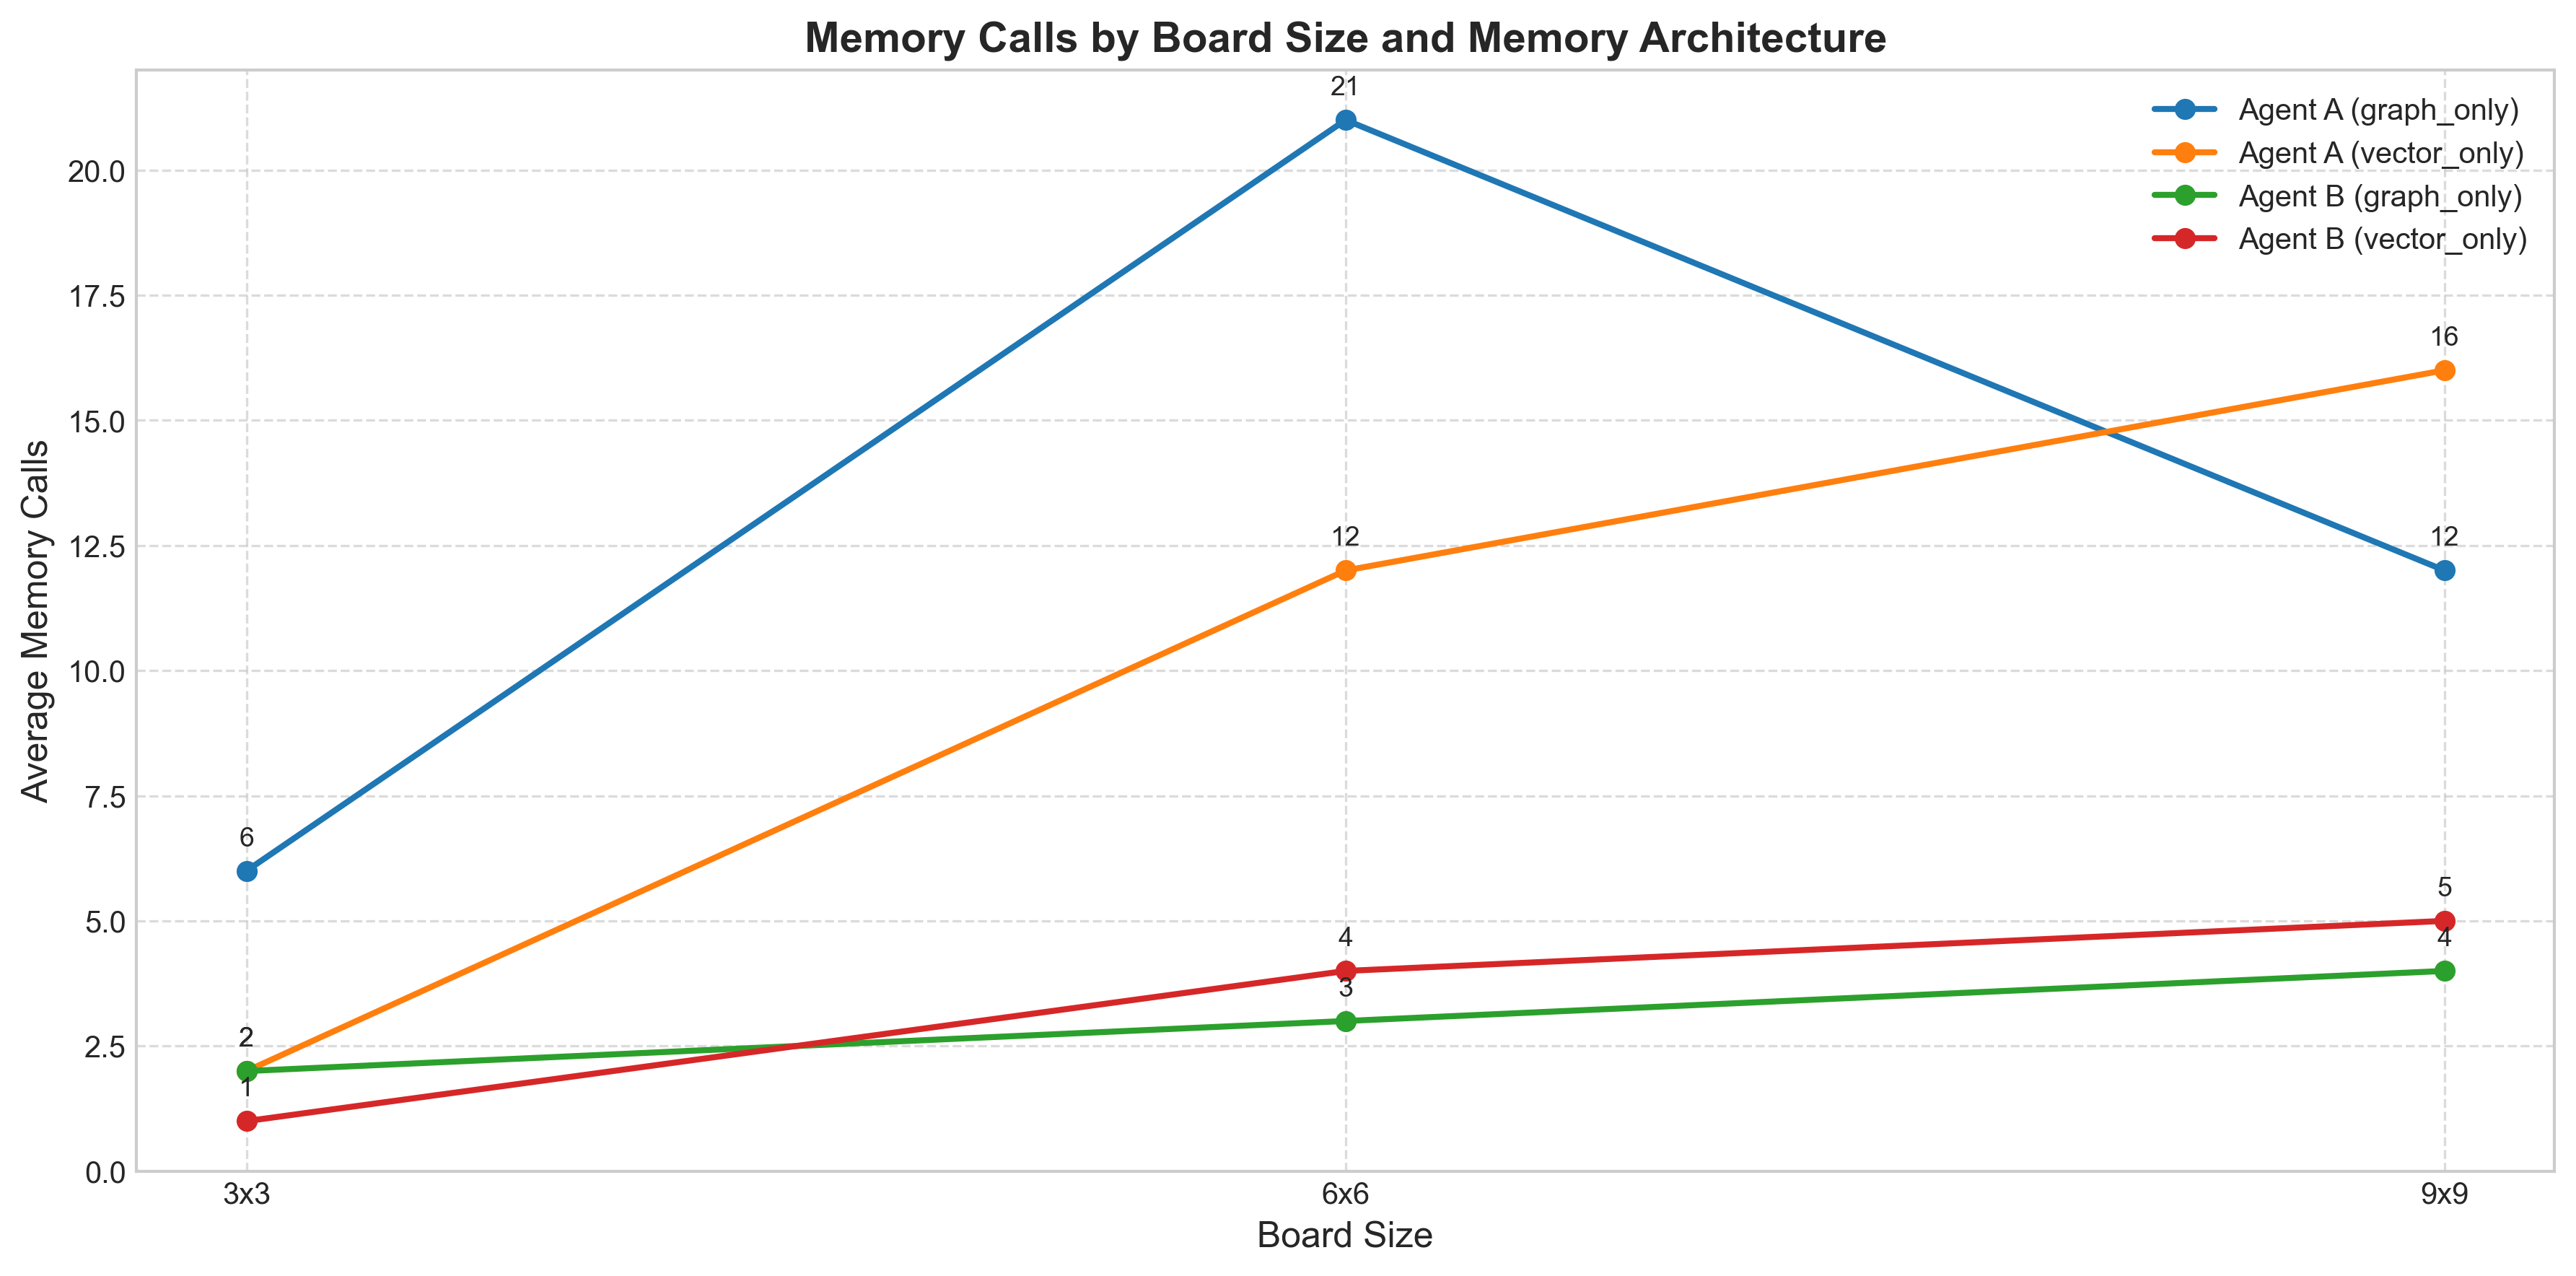
\includegraphics[width=0.7\textwidth]{figures/memory_calls_by_board_size.png}
\caption{Memory calls by board size and memory type. Agent A (solid lines) makes consistently more calls than Agent B (dashed lines) across all settings.}
\label{fig:memory_calls}
\end{figure}

These findings align with \textbf{H2.2}, indicating that memory demand grows with complexity but is mediated by both architecture and agent objective.

\begin{figure}[ht]
    \centering
    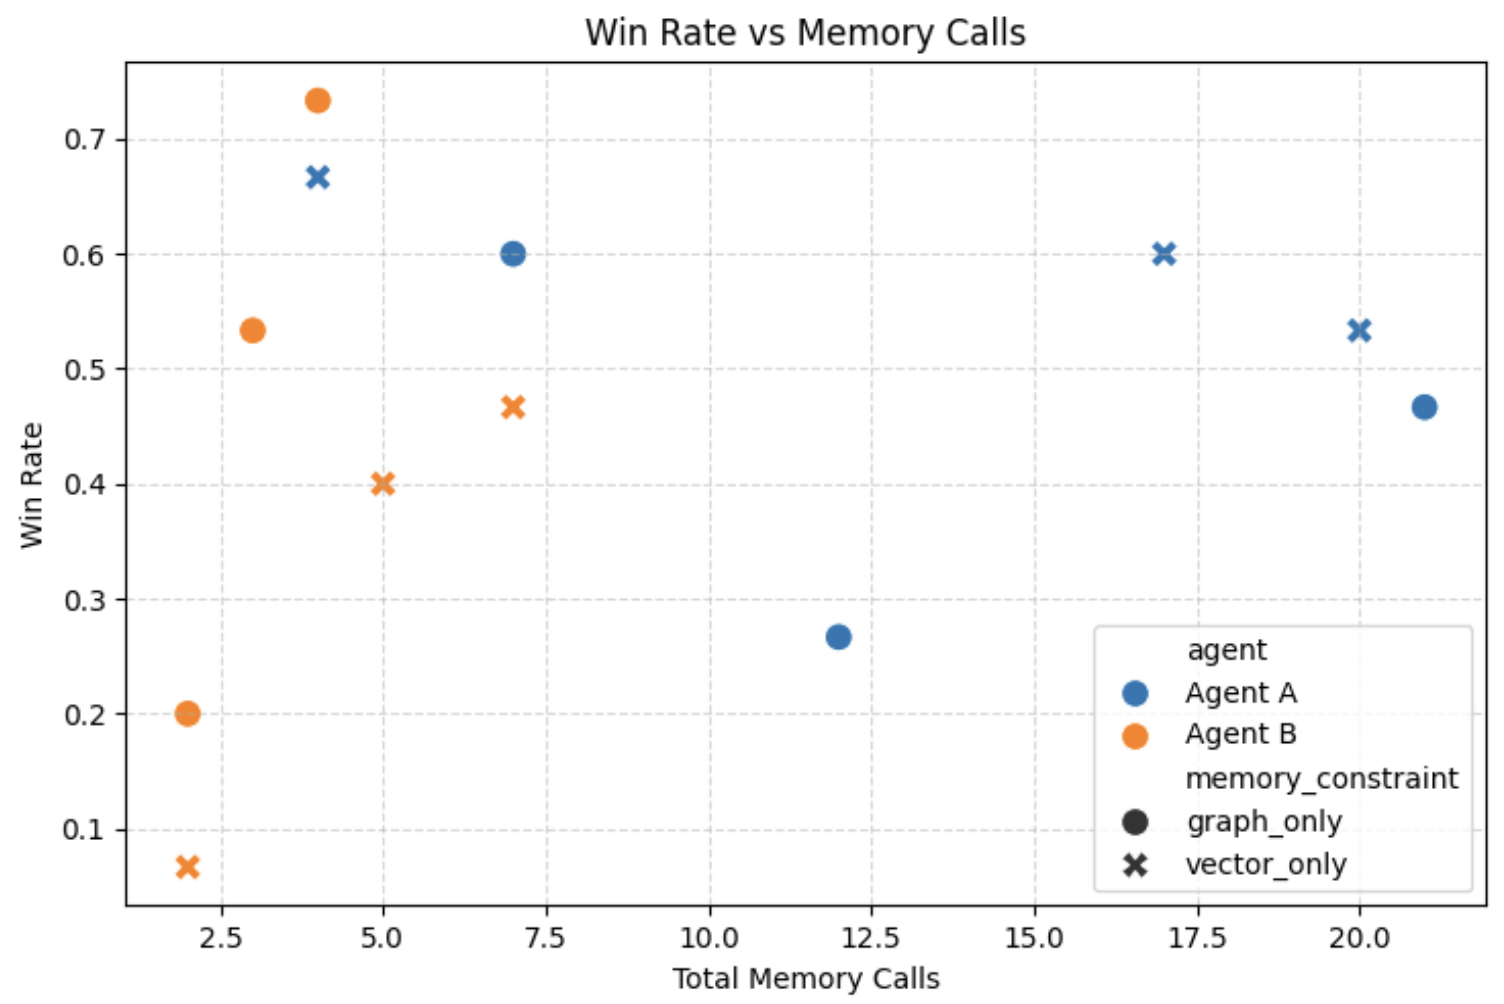
\includegraphics[width=0.6\textwidth]{figures/analysis/scatter_win_rate.png}
    \caption{Relationship between total memory calls and win rate across agents and memory configurations. Higher memory calls do not consistently correlate with better performance, highlighting diminishing returns in certain configurations.}
    \label{fig:scatter_win_rate}
    \end{figure}

\subsubsection{RQ3: Memory Efficiency $\neq$ Win Rate}

To investigate whether more efficient memory usage correlates with better performance, we examine the relationship between memory usage patterns and win rates across all memory conditions. Each point in our analysis represents one agent-memory-board configuration.

Our analysis reveals that higher memory usage does not necessarily translate to better performance. Agent A (blue) consistently makes more memory calls than Agent B (orange) across configurations, often 2–4 times more, reflecting their distinct prompt framings: Agent A focuses solely on win maximization, while Agent B accounts for token efficiency.

However, as shown in Figure~\ref{fig:scatter_win_rate}, \textbf{more memory calls do not guarantee higher win rates}. While Agent A (blue) often makes more memory calls (ranging from 7 to over 20 per game), the corresponding win rates remain variable, fluctuating between 0.28 and 0.6. In contrast, Agent B (orange) achieves higher and more stable win rates (0.5 to 0.73) with fewer memory calls (2 to 6 per game). This suggests diminishing returns for Agent A's aggressive retrieval patterns—beyond a certain point, increasing memory calls does not yield proportional performance gains.

Conversely, Agent B maintains \textbf{competitive or superior win rates with consistently fewer memory calls}, particularly in complex environments like $9\times9$. This reinforces the insight that \textbf{memory quality, not quantity}, drives success—targeted, efficient memory use outperforms brute-force retrieval strategies. Further examining token usage in Figure~\ref{fig:memory_efficiency_tradeoff}, we see similar patterns where Agent A's higher token consumption doesn't consistently translate to proportional performance gains.

In sum, RQ3 is supported: \textbf{memory quantity alone is not a reliable predictor of agent success}. Instead, strategic selectivity and retrieval relevance shape effective memory use.

\subsubsection{RQ4: Memory Efficiency Tradeoff}

Compared to baseline performance, constrained memory settings reveal that while memory augmentation can significantly improve win-token efficiency and reasoning stability in larger state spaces (especially for Agent A), the choice of memory architecture (Graph vs. Vector) remains critical.

\begin{figure}[ht]
\centering
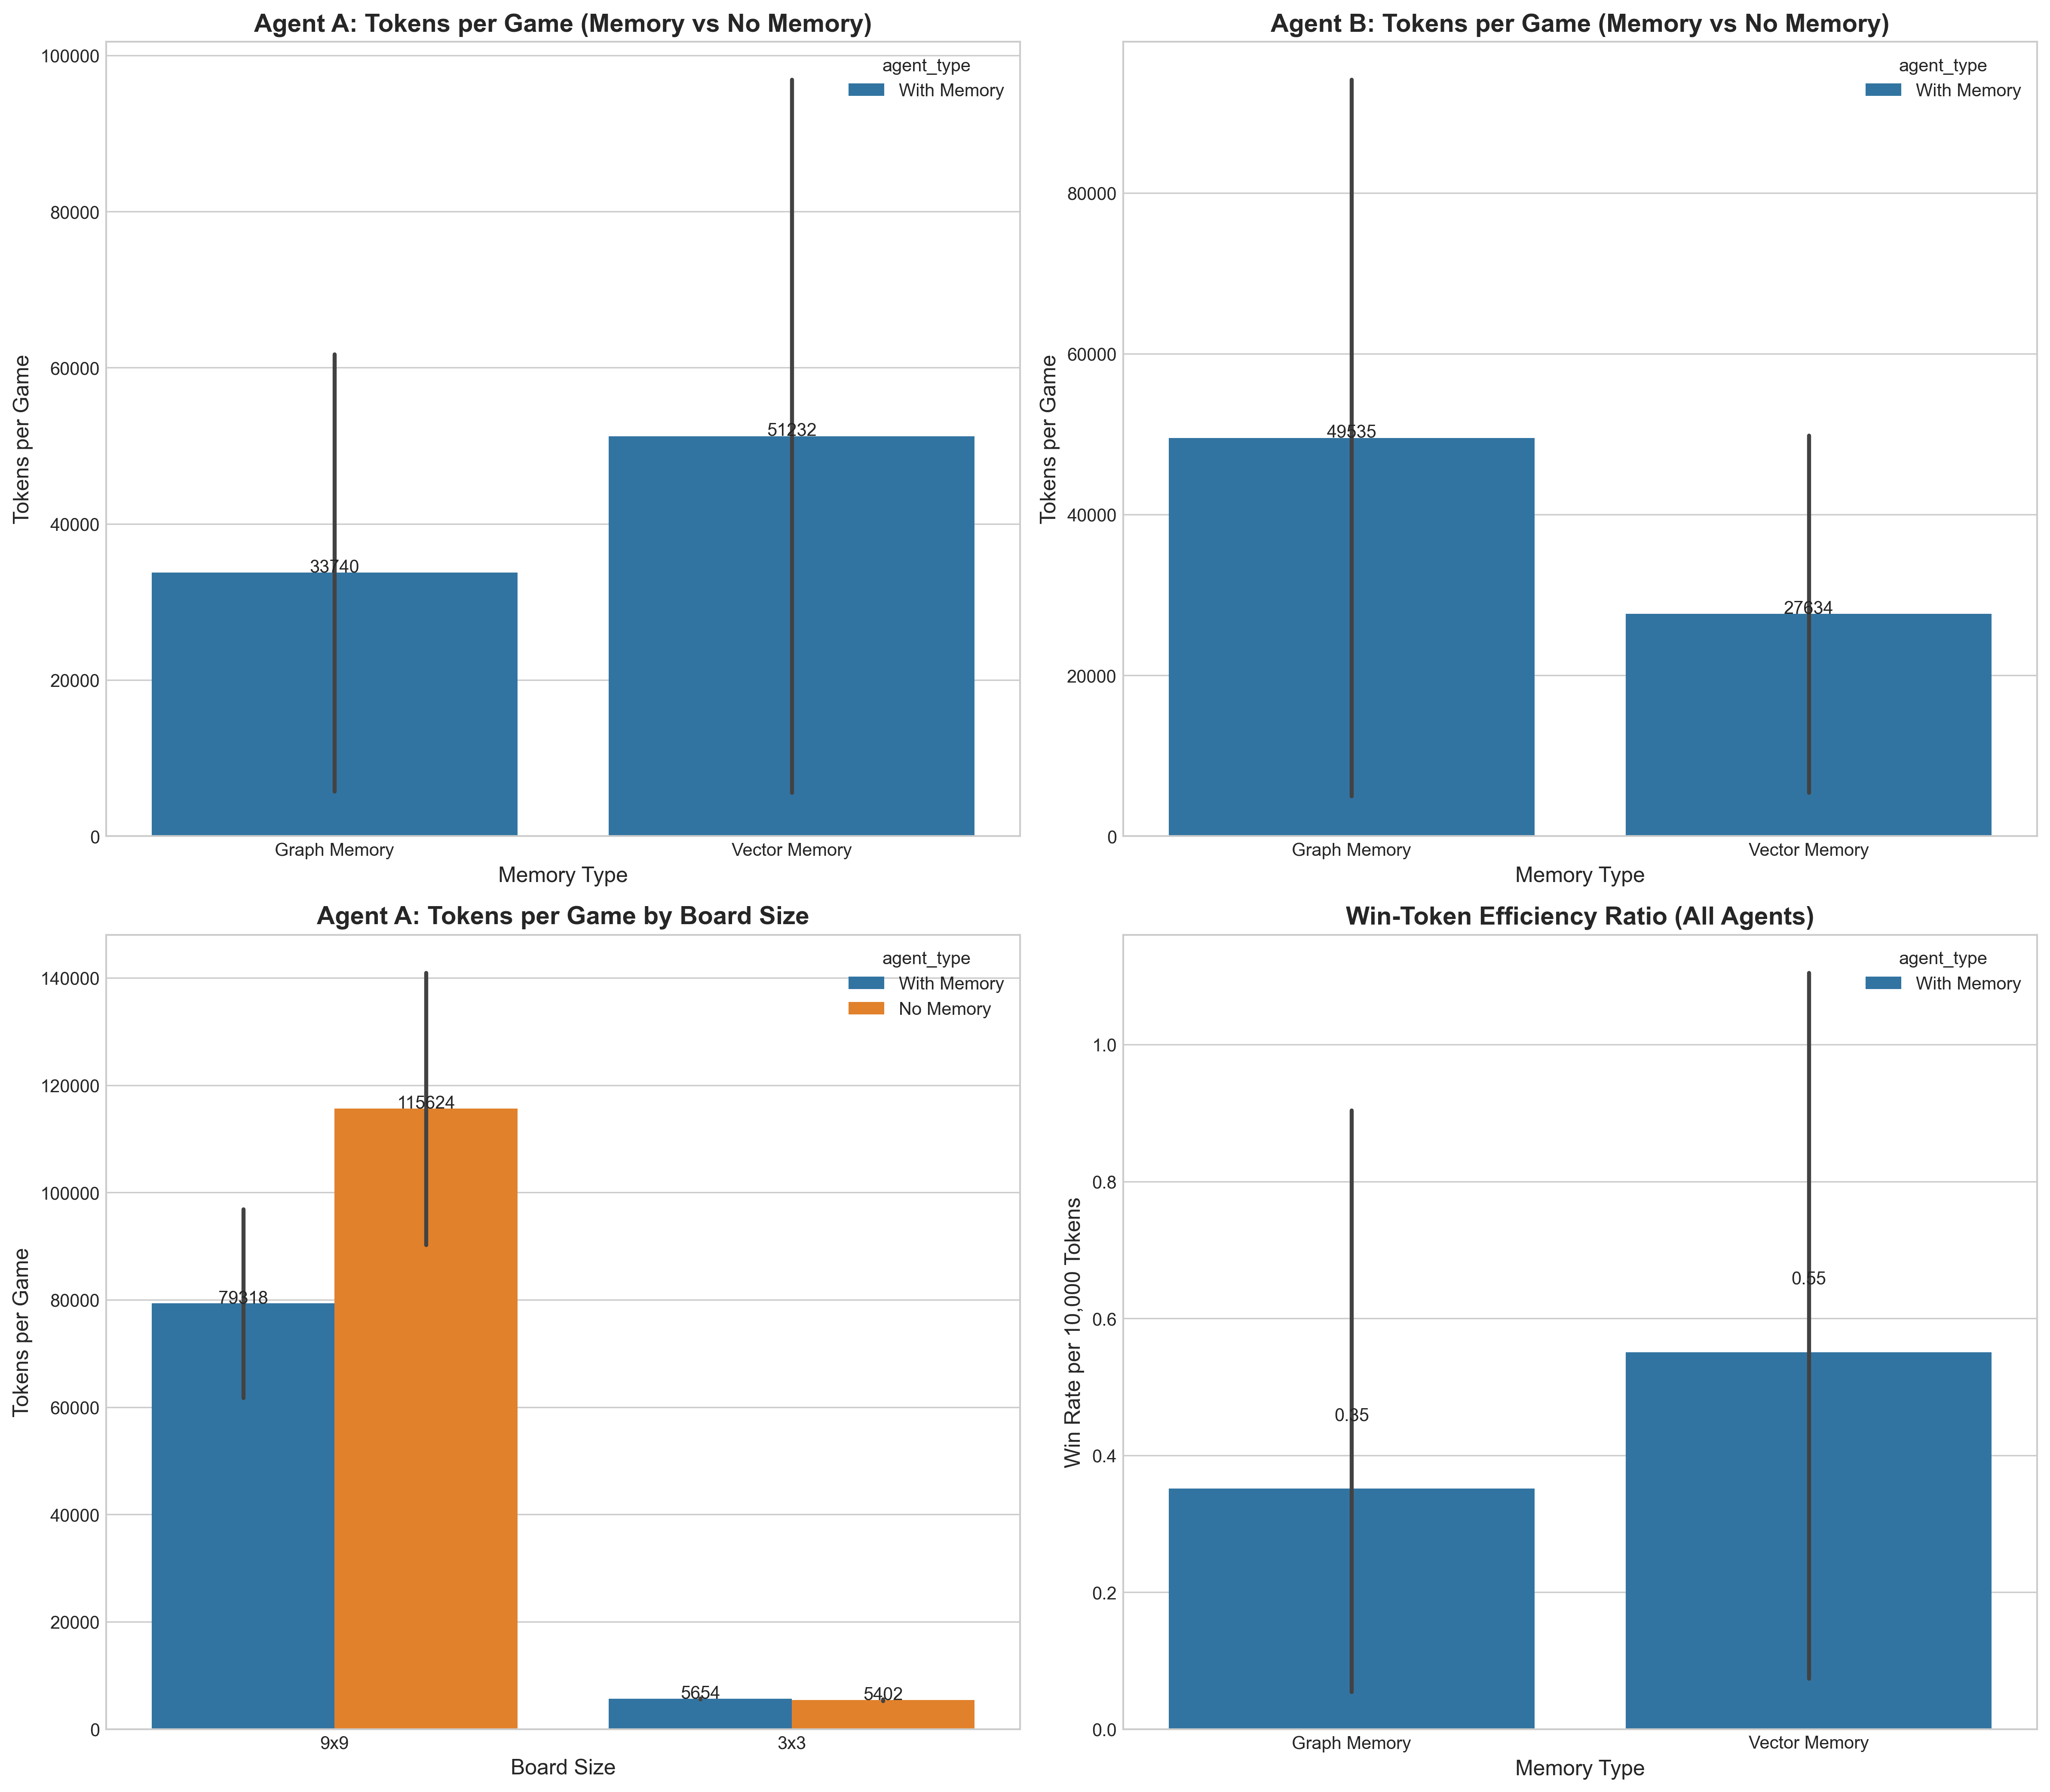
\includegraphics[width=0.7\textwidth]{figures/memory_baseline/memory_token_efficiency.png}
\caption{Win-token efficiency ratios (down right) and Agent A's token usage per game by board size (down left). Highlights the tradeoff between performance gains and computational cost across memory conditions.}
\label{fig:memory_efficiency_tradeoff}
\end{figure}

As shown in Figure~\ref{fig:memory_efficiency_tradeoff}, VectorMemory consistently enhances win-token ratios relative to baseline, particularly in $9\times9$ environments where reasoning demands are high. In contrast, GraphMemory often underperforms, exhibiting higher token usage without proportional gains in win rates. This contrast highlights that memory presence alone is insufficient—architecture alignment is essential to overcoming LLM scaling limits and ensuring efficient resource use.

This finding reinforces RQ4, demonstrating that effective memory augmentation depends not only on adding memory but selecting architectures that balance retrieval utility and computational cost.

\subsection{RQ5: Adaptive Memory Experiments}

In the adaptive setting, agents were granted full access to all memory types—GraphMemory, VectorMemory, and SemanticMemory. This experiment aimed to assess whether agents could autonomously adapt both \textbf{when} to use memory and \textbf{which} memory type to select based on task complexity and internal objectives.

\paragraph{Memory Type Preferences.}
Figure~\ref{fig:adaptive_memory_type} illustrates the distribution of memory type selections per agent. Contrary to patterns observed in constrained settings, both agents exhibited a strong bias toward \textbf{GraphMemory} across all board sizes. Notably, \textbf{Agent B} also leveraged \textbf{SemanticMemory} for over 30\% of its memory calls, despite its placeholder status. This emergent behavior suggests that Agent B may interpret SemanticMemory as a cost-effective fallback or conceptual retrieval tool. \textbf{VectorMemory}, which dominated in constrained experiments, played a secondary role, especially for Agent A.

\begin{figure}[ht]
\centering
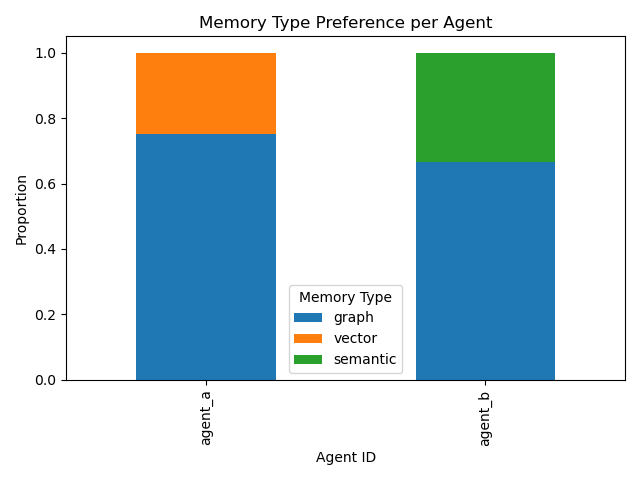
\includegraphics[width=0.55\textwidth]{figures/adaptive/memory_type_preference.png}
\caption{Memory type distribution across board sizes in adaptive mode. Both agents show a preference for GraphMemory, with Agent B also utilizing SemanticMemory.}
\label{fig:adaptive_memory_type}
\end{figure}

\paragraph{Memory Call Frequency.}
Figure~\ref{fig:adaptive_memory_frequency} reveals a \textbf{non-linear memory engagement profile}. \textbf{Agent A} exhibited peak memory calls at $6\times6$ boards, followed by a reduction at $9\times9$, whereas \textbf{Agent B} consistently minimized memory usage across all settings. This divergence suggests that Agent A's retrieval strategies are sensitive to task complexity but prone to saturation in larger state spaces. Agent B, in contrast, maintained highly selective engagement, likely due to internalized cost constraints.

\begin{figure}[ht]
\centering
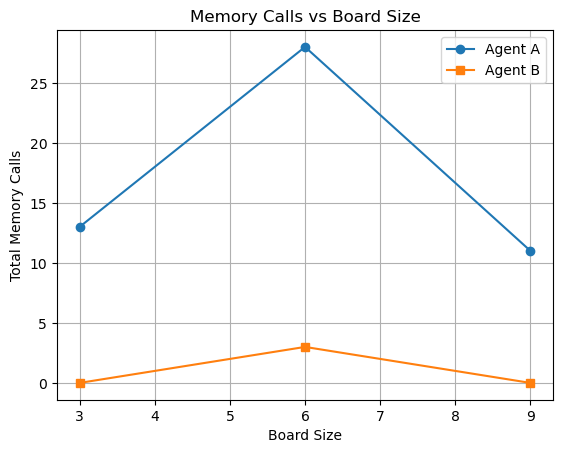
\includegraphics[width=0.55\textwidth]{figures/adaptive/memory_calls_vs_board_size.png}
\caption{Average memory calls per game across board sizes. Agent A shows peak usage at $6\times6$ followed by a reduction, while Agent B maintains minimal memory engagement.}
\label{fig:adaptive_memory_frequency}
\end{figure}

\paragraph{Token Usage and Efficiency.}
Token consumption trends deviated from expectations. As shown in Figure~\ref{fig:adaptive_token_usage}, \textbf{Agent B} incurred \textbf{higher token costs} than Agent A, particularly on $9\times9$ boards. This inversion suggests that despite fewer memory calls, Agent B's reasoning paths may be more verbose or reliant on token-intensive computations—potentially tied to SemanticMemory's overhead.

\begin{figure}[ht]
\centering
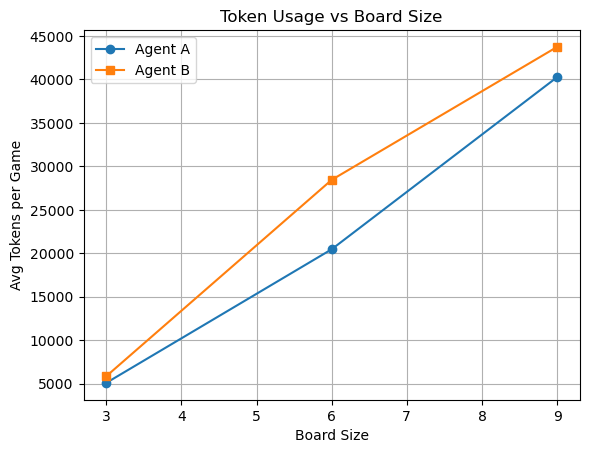
\includegraphics[width=0.55\textwidth]{figures/adaptive/token_usage_vs_board_size.png}
\caption{Token usage across board sizes in adaptive mode. Unexpectedly, Agent B shows higher token consumption on complex boards despite fewer memory calls.}
\label{fig:adaptive_token_usage}
\end{figure}

\paragraph{Performance Tradeoffs.}
Figure~\ref{fig:adaptive_win_rate} shows that \textbf{Agent A consistently outperformed Agent B in win rate} across all board sizes. Remarkably, this advantage was achieved with \textbf{lower token usage}, inverting the expected efficiency-performance tradeoff. Agent A's selective but effective engagement with GraphMemory appears to yield better outcomes than Agent B's cautious but costlier strategies.

\begin{figure}[ht]
\centering
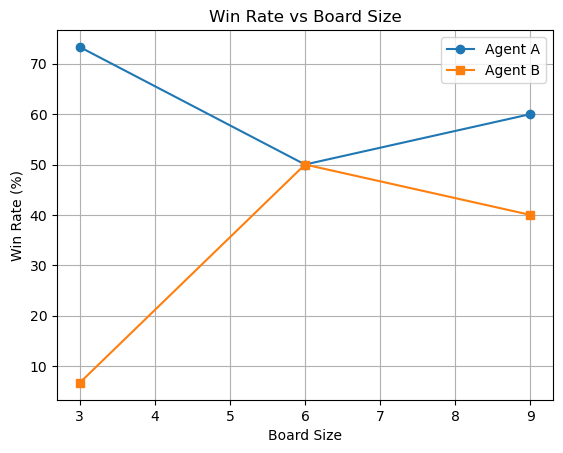
\includegraphics[width=0.55\textwidth]{figures/adaptive/win_rate_vs_board_size.png}
\caption{Win rates across board sizes in adaptive mode. Agent A maintains superior performance with lower token costs, contrary to expectations.}
\label{fig:adaptive_win_rate}
\end{figure}

These findings refine our understanding of \textbf{H3}, demonstrating that:
\begin{enumerate}[leftmargin=*,nosep]
\item Agents do autonomously adapt memory usage, but \textbf{adaptivity alone does not ensure efficiency};
\item Memory architecture preferences and cost models co-determine whether adaptive strategies yield optimal tradeoffs.
\end{enumerate}

\paragraph{Summary.}
The adaptive experiments highlight that while agents flexibly adjust memory use, \textbf{architecture alignment remains critical}. \textbf{Agent A's} reliance on GraphMemory delivered superior \textbf{win-token tradeoffs}, outperforming Agent B's more conservative, yet less efficient approach. This suggests that success in adaptive settings hinges not just on \textbf{when} or \textbf{how much} memory is used, but on \textbf{choosing the right memory architecture} for the task at hand.

\section{Discussion}

\subsection{Implications for Memory Architecture Design}

Our findings carry several implications for the design of memory systems in LLM agents. First, the consistent superiority of \textbf{VectorMemory} across increasing task complexity suggests that \textbf{fuzzy retrieval mechanisms} generalize more effectively than structured, relational storage in high-variance environments. While \textbf{GraphMemory} offers clear benefits in smaller, well-structured settings (e.g., the $3 \times 3$ board), its performance degrades sharply as the environment scales. This indicates that graph-based relational reasoning—while interpretable—faces scalability limits when the number of potential state transitions explodes. In contrast, the pattern-matching capabilities of vector-based retrieval, powered by latent-space embeddings, allow agents to flexibly navigate large and sparsely populated state spaces. This suggests that for agents operating in open-ended or poorly structured environments, \textbf{vector-based memory architectures may offer more robust scalability}, a principle likely to extend beyond TicTacToe.

Second, our experiments highlight the subtle but significant influence of \textbf{prompt framing} in shaping agent behavior, even when optimization objectives remain formally identical. Though both agents were tasked with maximizing win rate while minimizing token use, Agent B's repeated reminders about token costs led to \textbf{emergent resource-conscious strategies}—characterized by lower memory usage frequency and greater token efficiency. This divergence demonstrates that \textbf{prompt design acts as a soft constraint} on LLM agents, shaping not only local decision-making but broader strategic patterns over time. For developers of cognitive architectures and LLM-based planning agents, this finding underscores the need to carefully craft system-level prompts, as these seemingly minor choices can have outsized effects on agent behavior.

Finally, the tradeoff between \textbf{aggressiveness} and \textbf{efficiency} that emerged across our agents offers further insights for LLM-based agent design. Agent A's strategy—driven solely by win maximization—led to more frequent memory use, but with diminishing returns at scale. Agent B, by contrast, balanced token costs and selectively used memory, yielding \textbf{better performance retention} and \textbf{higher win-rate-to-token ratios} in larger environments. This suggests that, especially in resource-constrained settings, \textbf{conservative memory strategies} may support more scalable and robust agent performance.

\subsection{Limitations and Reflection}

While our study provides valuable insights into LLM-agent memory strategies, several limitations constrain the generalizability and depth of our conclusions:

First, our experiments are confined to TicTacToe, even though we scale the board size to increase complexity. While this scaling expands the state space, TicTacToe remains a deterministic, turn-based environment with relatively simple strategy spaces. Richer domains—such as Connect4, multi-agent coordination, or open-ended dialogue—may impose different demands on memory systems.

Second, our implementation of SemanticMemory was limited in scope and optimization. Though accessible in adaptive experiments and surprisingly leveraged by Agent B, it remained a placeholder without robust retrieval or storage mechanisms. This limits our ability to evaluate how agents might fully integrate conceptual memory alongside structured (GraphMemory) and fuzzy (VectorMemory) systems.

Third, our adaptive experiments, while revealing, were conducted with limited sample sizes due to computational constraints. This led to noisier trends in memory type selection and token efficiency, particularly in adaptive scenarios where agents' preferences diverged from constrained expectations (e.g., GraphMemory dominance over VectorMemory). A larger experimental pool could yield clearer patterns.

Fourth, our agents operated under fixed prompting-based objectives, with no reinforcement learning (RL) or external reward signals. This limits their capacity to adaptively refine memory usage strategies over time based on cumulative success or cost-efficiency. Without RL, agents cannot fully explore long-term tradeoffs or develop meta-memory behaviors such as schema evolution or memory compression.

Finally, while our memory operations include \texttt{store}, \texttt{retrieve}, and \texttt{updateSchema}, the meta-memory reasoning capacities of agents were underutilized. Schema updates were rare, suggesting that agents did not engage deeply with memory structure optimization. Future work could explore more advanced memory lifecycle management, such as forgetting, compression, or restructuring.

\subsection{Future Directions}

Our findings point to several promising extensions:
\begin{enumerate}
    \item Extend to longer-horizon and richer environments. Moving beyond TicTacToe to domains like Connect4, strategy games, or multi-agent dialogue systems would better test memory scalability, decision-making under uncertainty, and long-term planning.
    
    \item Enhance SemanticMemory and multi-modal memory integration. Developing a more sophisticated SemanticMemory with true conceptual retrieval could reveal whether agents can balance structured, fuzzy, and conceptual memories based on context. This would enable deeper investigation into adaptive memory selection and hierarchical reasoning.
    
    \item Incorporate reinforcement learning (RL) for memory optimization. While our study shaped agent behavior through prompting alone, RL could enable agents to learn memory usage policies, optimizing when to retrieve, store, or compress based on long-term rewards. RL-driven meta-strategy learning might foster more nuanced memory management, particularly in resource-constrained settings.
    
    \item Explore dynamic $\lambda$ tuning. Allowing agents to adjust their win-token tradeoff parameter ($\lambda$) during training could yield more adaptive behaviors, reflecting real-world scenarios where efficiency pressures vary over time.
    
    \item Investigate meta-memory mechanisms. Future work could explore memory compression, schema optimization, forgetting, and other lifecycle management techniques, enabling agents to manage memory as a bounded resource over longer interactions.
\end{enumerate}

Together, these directions can advance our understanding of how LLM agents can autonomously manage complex memory systems, balancing scalability, efficiency, and adaptability in increasingly dynamic environments.

\section{Conclusion}

This study investigated how LLM agents, equipped with modular external memory systems, adapt their memory strategies under differing objectives and task complexities. By pairing GPT-4o-mini with GraphMemory and VectorMemory in self-play TicTacToe across scaled board sizes, we systematically evaluated how memory architecture and prompt framing shape agent behavior.

Our key findings include:

\begin{itemize}[leftmargin=*,nosep]
\item \textbf{VectorMemory scales more robustly} than GraphMemory, maintaining higher performance retention and win-token efficiency as state space complexity increases.
\item \textbf{Agent objectives significantly influence memory usage}, with token-aware agents (Agent B) demonstrating more selective and efficient strategies than win-maximizing agents (Agent A), despite sharing formal optimization goals.
\item \textbf{More memory usage does not always yield better performance}; targeted, efficient retrieval—rather than aggressive, high-frequency memory calls—proves crucial, especially under resource constraints.
\end{itemize}

These insights highlight that memory augmentation alone is insufficient: effective systems require alignment between memory architecture and agent objectives, as well as mechanisms to balance retrieval utility and computational cost.

Looking forward, enriching memory architectures (including SemanticMemory), integrating reinforcement learning for memory optimization, and scaling to longer-horizon environments offer exciting paths for enhancing LLM-based agents' reasoning, adaptability, and resource efficiency. These advances can drive the development of more robust, scalable agents capable of operating across complex decision spaces.

% Fix for bibliography processing
\bibliographystyle{plainnat}
\bibliography{bibliography}

\end{document}
